
%(BEGIN_QUESTION)
% Copyright 2014, Tony R. Kuphaldt, released under the Creative Commons Attribution License (v 1.0)
% This means you may do almost anything with this work of mine, so long as you give me proper credit

Old vacuum-tube based electronic circuits often required several different voltage levels for proper operation.  An easy way to obtain these different power supply voltages was to take a single, high-voltage power supply circuit and ``divide'' the total voltage into smaller divisions.

These voltage divider circuits also made provision for a small amount of ``wasted'' current through the divider called a {\it bleeder} current, designed to discharge the high voltage output of the power supply quickly when it was turned off.

Design a high-voltage divider to provide the following loads with their necessary voltages, plus a ``bleeder'' current of 5 mA (the amount of current going through resistor R4):

$$\includegraphics[width=15.5cm]{i01137x01.eps}$$

\underbar{file i01137}
%(END_QUESTION)





%(BEGIN_ANSWER)

The key to calculating all resistor values is to determine how much voltage each one must drop and how much current each one must carry.  The current question may be answered by applying Kirchhoff's Current Law (KCL) to each of the nodes in the circuit, while the voltage question may be answered by calculating the voltage difference between each pair of supply lines to the tube circuit.

\begin{itemize}
\item{} $R_1 =$ 3.25 k$\Omega$ 
\item{} $R_2 =$ 11 k$\Omega$
\item{} $R_3 =$ 3.67 k$\Omega$
\item{} $R_4 =$ 9 k$\Omega$
\end{itemize}

%(END_ANSWER)





%(BEGIN_NOTES)

Be sure to ask your students {\it how} they obtained the solution to this problem.  If no one was able to arrive at a solution, then present the following technique: simplify the problem (fewer resistors, perhaps) until the solution is obvious, then apply the same strategy you used to solve the obvious problem to the more complex versions of the problem, until you have solved the original problem in all its complexity.

%INDEX% Electronics review: series-parallel circuits

%(END_NOTES)


